\chapter{Evaluation and data acquisition}
\section{Data Acquisition}
For measurement on the true surface topography of snake sheds, samples are stuck on glass plates using double face tape, the animal was pushed up below a hollowed plate letting the skin emerging from the top of the plate using an atomic force microscope (AFM). An AFM is a microscope that uses a tiny probe mounted on a cantilever to scan the surface of an object. The probe is extremely close tobut does not touch the surface. As the probe traverses the surface, attractive and repulsive forces arising between it and the atoms on the surface induce forces on the probe that bend the cantilever. The amount of bending is measured and recorded, providing a map of the atoms on the surface. Atomic force microscopes is a very high-resolution type of scanning probe microscopy, with demonstrated resolution on the order of fractions of a nanometer, more than 1000 times better than the optical diffraction limit.

\section{Diffraction Gratings}
An idealised grating like in figure $\ref{fig:lighthitsgrating}$ is made of a very large number of parallel, evenly spaced slits in an opaque sheet. Typically, it would have about 10,000 slits. In order to cause diffraction, the spacing between slits must be wider than the wavelength of the incoming light beam. Each slit in the grating acts as a quasi point light source from which light propagates in all directions. Figure $\ref{fig:spectometer}$ illustrates this behaviour for a monochromatic light source passing through a grating and shows that the the outgoing angle will be different from the incident angle. Hence, the diffracted light $\ref{diffractiondeff}$ is composed of the sum of interfering wave components emanating from each slit in the grating.

\begin{figure}[H]
  \centering
  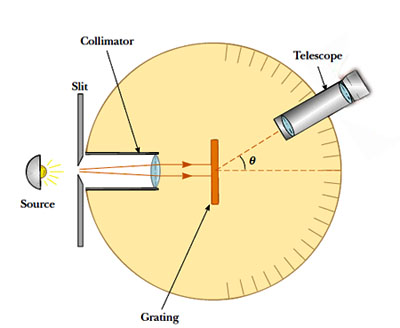
\includegraphics[scale=0.7]{evaluation/spectrometer.jpg}
  \caption{Spectometer: When a beam of monochromatic light passes through a grating placed in a spectrometer, images of the sources can be seen through the telescope at different angles.}
\label{fig:spectometer}
\end{figure}

Suppose monochromatic light is directed at the grating parallel to its axis as shown in figure $\ref{fig:spectometer}$. Let the distance between successive slits be equal $d$.

\begin{figure}[H]
  \centering
  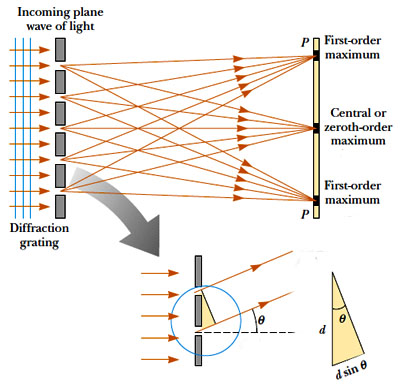
\includegraphics[scale=0.7]{evaluation/grating2.jpg}
  \caption{Light directed to parallel to grating:}
  \label{fig:lighthitsgrating}
\end{figure}

The diffraction pattern on the screen is the result of the combined effects of diffraction and interference. Each slit causes diffraction, and the diffracted beams in turn interfere with one another to produce the pattern. The path difference between waves from any two adjacent slits can be found by dropping a perpendicular line between the parallel waves. By geometry, this path difference is $d sin(\theta)$. If the path difference equals one wavelength or some integral multiple of a wavelength, waves from all slits will be in phase and a bright line will be observed at that point. Therefore, the condition for maxima in the interference pattern at the angle $\theta$ is: 

\begin{equation}
 d sin(\theta) = m \lambda 
\label{eq:simplegratingequation}
\end{equation}

where $m \in \mathds{N}_0$ is the order of diffraction.

Because $d$ is very small for a diffraction grating, a beam of monochromatic light passing through a diffraction grating is splitted into very narrow bright fringes at large angles $\theta$.

\begin{figure}[H]
  \centering
  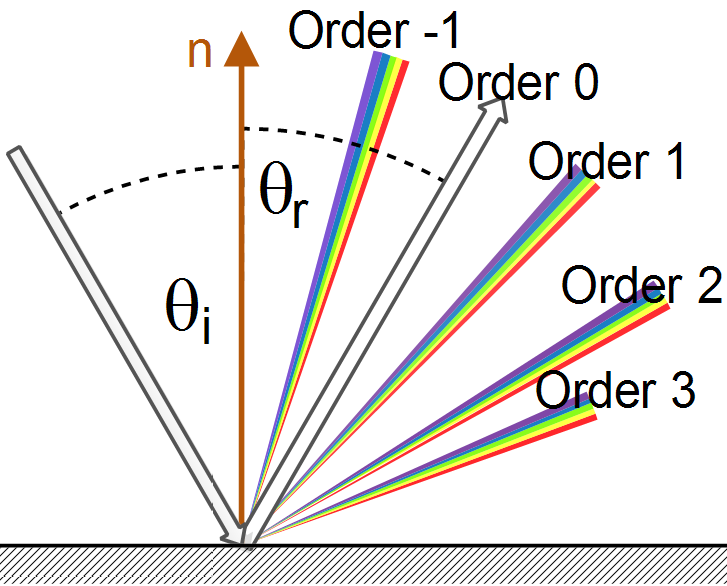
\includegraphics[scale=0.7]{evaluation/GratingSurface.png}
  \caption{Different Orders of diffraction}
\label{fig:gratingdiffractionorders}
\end{figure}

When a narrow beam of white light is directed at a diffraction grating along its axis, instead of a monochromatic bright fringe, a set of colored spectra are observed on both sides of the central white band as shown in figure $\ref{fig:gratingdiffractionorders}$.

\begin{figure}[H]
  \centering
  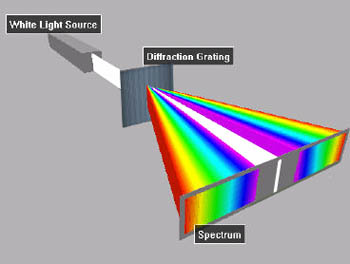
\includegraphics[scale=0.7]{evaluation/coloredspectrum.jpg}
  \caption{White Light beam causes coloured diffraction spectra}
  \label{fig:diffractionSpectrum}
\end{figure}

Since the angle $\theta$ increases with wavelength $\lambda$, red light, which has the longest wavelength, is diffracted through the largest angle. Similarly violet light has the shortest wavelength and is therefore diffracted the least. This relationship between angle and wavelength is illustrated in figure $\ref{fig:diffractionSpectrum}$. Thus, white light is split into its component colors from violet to red light. The spectrum is repeated in the different orders of diffraction, emphasizing certain colors differently, depending on their order of diffraction like shown in figure $\ref{fig:gratingdiffractionorders}$. Note that only the zero order spectrum is pure white.  
Figure $\ref{fig:nslitdiffractionintensity}$ shows the relative intensity resulting when a beam of light hits a diffraction grating for different number of periods. From the graph we recognise that the more slits a grating has, the sharper more slopes the function of intensity gets. This is similar like saying that, the more periods a grating has, the sharper the diffracted color spectrum gets like shown in figure $\ref{fig:diffractionslits}$. 

\begin{figure}[H]
  \centering
  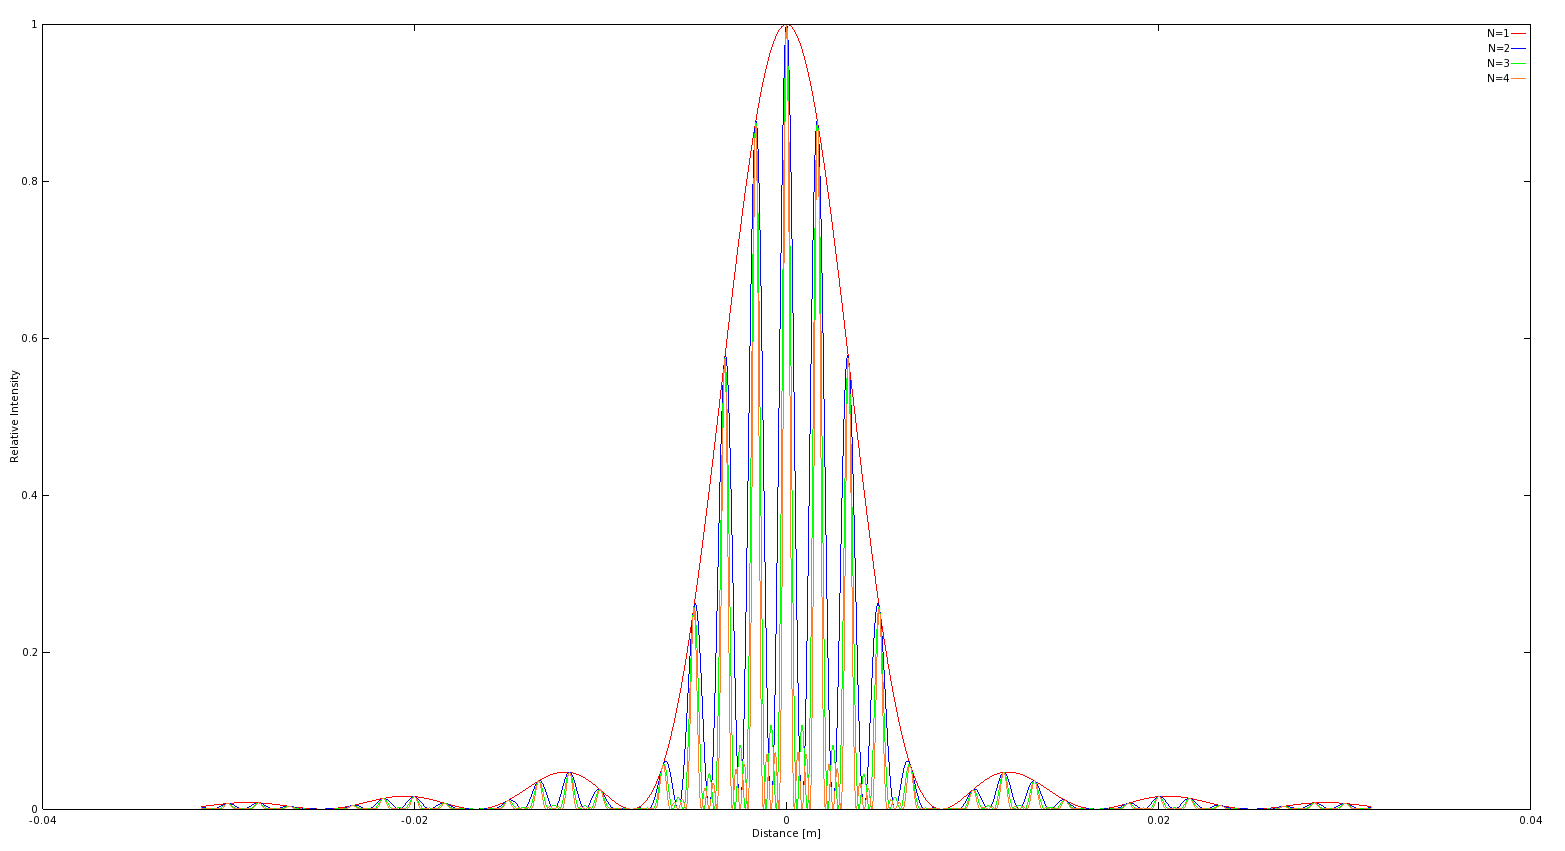
\includegraphics[scale=0.35]{evaluation/nslitdiffraction.png}
  \caption{Relative intensitiies of a diffracted beam of light at wavelength $\lambda=500nm$ on a grating for different number of periods $N$ width slit width of 30 microns and slit seperation of 0.15 mm each. The viewer is 0.5m apart from the grating.}
  \label{fig:nslitdiffractionintensity}
\end{figure}

\begin{figure}[H]
  \centering
  \subfigure[one slit]{
    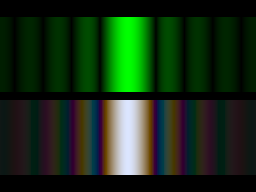
\includegraphics[scale=0.2]{evaluation/slits/spalt1.png}
    \label{fig:diffractionSlits1}
  }

~
  \subfigure[seven slits]{
    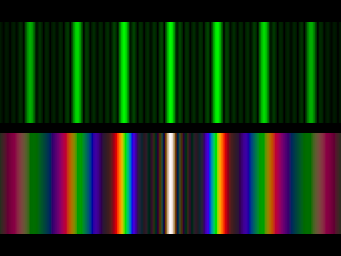
\includegraphics[scale=0.2]{evaluation/slits/spalt07.png}
    \label{fig:diffractionSlits7}
  }
  
  
\caption{Difference of diffraction pattern between a monochromatic (top) and a white (bottom) light spectra for different number of slits.}
\label{fig:diffractionslits}
\end{figure}

\section{Evaluation}

\begin{figure}[H]
  \centering
  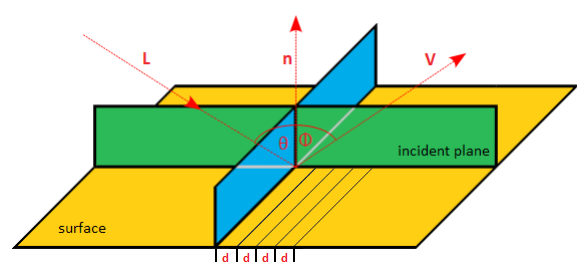
\includegraphics[scale=0.65]{evaluation/evalsetup.png}
  \caption{Experimental setup for evaluation: A light beam with direction $L$ hits the surface, representing a grating pattern with periodicity $d$, at the incident plane relative to the surface normal $n$ at angle $\theta$ and emerges at angle $\phi$ with direction $V$.}
  \label{fig:experimentalsetup}
\end{figure}

The physical reliability of our BRDF models has been verified by applying those on various patches which are a synthetic blazed grating, an Elaphe and a Xenopeltis snake shed sample patch. We compared the resulting response against the response resulting by the grating equation, which models the relationship between the grating spacing and the angles of the incident and diffracted beams of light. Figure $\ref{fig:experimentalsetup}$ illustrates the geometrical setup for our evaluation approach: A monochromatic beam of light with wavelength $\lambda$ hits a surface with periodicity $d$ at an angle $\theta$ relative to the normal $n$ along its incident plane. The beam emerges from the surface at the angle $\phi$. 

\begin{figure}[H]
  \centering
  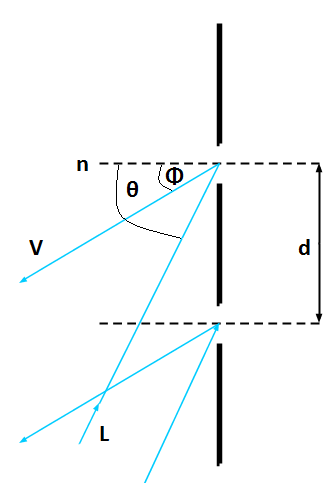
\includegraphics[scale=0.45]{evaluation/reflgrating.png}
  \caption{Reflecting grating: When the incident light direction is not parallel to its axis at the grating, there is another $sin(\phi)$ involved. See also the grating equation $\ref{eq:gratingeq}$.}
  \label{fig:reflgrating}
\end{figure}

The maximum in intensity is given by the grating equation derived from the equation $\ref{eq:simplegratingequation}$ following figure $\ref{fig:reflgrating}$: 

\begin{equation}
  sin(\theta) = sin(\phi) + \frac{m \lambda}{d}
\label{eq:gratingeq}
\end{equation}

In our evaluation we are interested in the first order diffraction, i.e. m equals one which. We further assume that the incident light direction $\omega_i$ is given. In contrast the direction of the reflected wave $\omega_r$ is not given.
In Mathematics, a three dimensional direction vector is fully defined by two two angles, i.e. it can be represented by spherical coordinates with radius $r = 1$. By convention, we denote those two vectors by $\theta$ and $\phi$ like in figure $\ref{fig:experimentalsetup}$. Hence, $\theta_i$, $\phi_i$ and $\phi_r$ are given constants whereas $\theta_i$ is a free parameter for our evaluation simulation. Therefore, we are going to compare the maxima for peak viewing angles corresponding to each wavelength using data produced by our method against the maxima resulting by the grating equation $\ref{eq:gratingeq}$.

\subsection{Precomputation}
\label{sec:evalprecomp}
For evaluation purposes we have implemented our brdf models in java. We once again use our geometrical setup as illustrated in figure $\ref{fig:geometricsetup}$ where $\theta_i$, $\phi_i$ and $\phi_r$ are provided as input values and $\theta_i$ is a free parameter. Within our evaluation we have set them to $\theta_i = 75$ $\phi_i = 0$ $\phi_r = 180$ degrees. The wavelength space $\Lambda$ and the range $\Theta$ of our free parameter $\theta_i$ are discretized in equidistant steps whereas their step sizes are given as input arguments for our Java program:

\begin{equation}
\Lambda = \{\lambda | \lambda = \lambda_{min} + k \cdot \lambda_{step}, \quad k \in \{0,..,C-1\}\}
\label{eq:lambdaspacesetup}
\end{equation}

where $\lambda_{step} = \frac{\lambda_{max}-\lambda_{min}}{C-1}$ and $C$ is the discretisation level of the lambda space. We similarly discretise the angle space by predefining an minimal and maximal angle boundary and $ceil(angMax - angMin) / angInc$ is the number of angles. Our Java BRDF model implementations are applied on the grid $[\Lambda, \Theta]$ and will store their spectral response in a matrix

\begin{equation} 
R = \{response(\lambda_i, \theta_{r}^{j}) | i \in Index(\Lambda), \quad j \in Index(\Theta)\}
\label{eq:responsematrix}
\end{equation}

We will plot this matrix and compare its graph against the grating equation for similar condition like in stated in algorithm $\ref{alg:evalmatlab}$.

\begin{algorithm}[H]
  \caption{Vertex diffraction shader}
  \begin{algorithmic}
    \State{load matrix $R$ $\ref{eq:responsematrix}$}
    \State $ \lambda_{count} = |\Lambda| $
    \State $ \lambda_{inc} = \frac{\lambda_{max}-\lambda_{min}}{\lambda_{count}}$
    \State $ \lambda = \lambda_{min} + \lambda_{inc} \cdot (-1+[1:\lambda_{count}])$
    \State $ [maxC maxI] = max(R)$
    \State $ viewAngForMax = angMin + angInc \cdot (maxI-1)$
    \State $ thetaV = asin \left( \frac{\lambda}{d} - \sin \left(  \frac{\theta_I \pi}{180} \right) \right) \cdot \frac{180}{\pi}$
    \State $ plot(\lambda, viewAngForMax)$
    \Comment{graph resulting by our brdf model}
    \State $ plot(lambda, thetaV)$
    \Comment{graph resulting by grating equation}
  \end{algorithmic}
\label{alg:evalmatlab}
\end{algorithm}

\subsection{Evaluation graphs}

\begin{figure}[H]
  \centering
  \subfigure[Blaze grating]{
    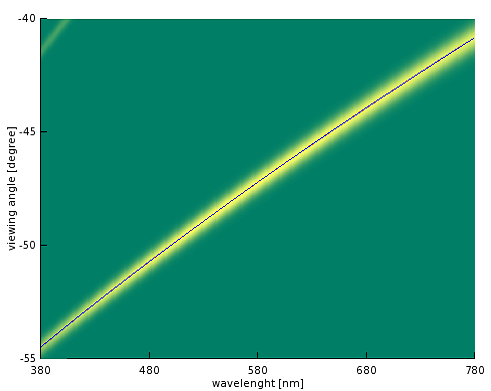
\includegraphics[scale=0.42]{evaluation/blazeHR.png}
    \label{fig:blazeval}
  }
~
  \subfigure[Xenopeltis grating]{
    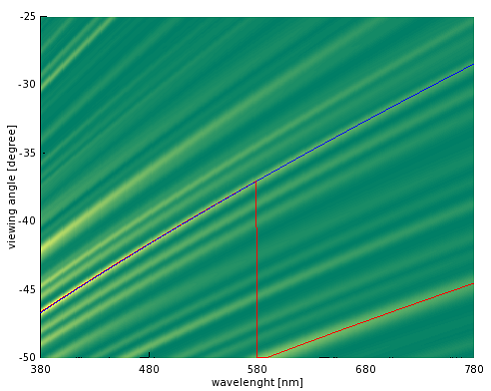
\includegraphics[scale=0.42]{evaluation/XenoHR.png}
    \label{fig:xenopeltiseval}
  }
~
\subfigure[Elaphe grating]{
  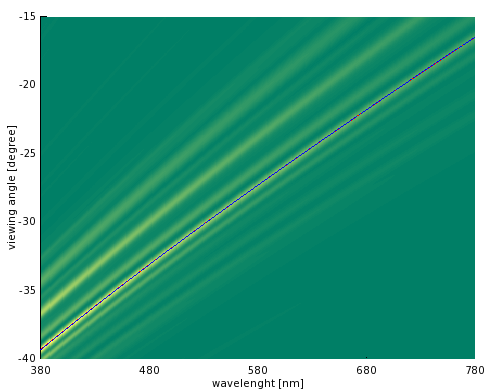
\includegraphics[scale=0.75]{evaluation/ElapheHR.png}
  \label{fig:elapheeval}
}

\caption{Reflectance obtained by using the shading approach described in algorithm $\ref{alg:fragmentshaderall}$ simulating a BRDF which models the effect of diffraction at different viewing angles over the spectrum of visible light.}

\label{fig:evaluationdiffshaderalllambda}
\end{figure}

In this section we discuss the quality of our BRDF models applied to different surface structures. For that purpose we compare the resulting relative reflectance computed as described in section $\ref{sec:evalprecomp}$ for each of our BRDF models to the idealized grating equation $\ref{eq:gratingeq}$. 

\begin{table}[H]
  \centering
  \begin{tabular}{| l | c | r |}
    \hline                       
    Patch & Mean[mm] & Variance[mm] \\
    \hline
    Blazed grating $\ref{fig:blazegratingpatch}$ & 2500.34 & 0.16 \\
    Elaphe grating $\ref{fig:elpahegratingpatch}$ & 1144.28 & 0.15 \\
    Xenopeltis grating $\ref{fig:xenogratingpatch}$ & 1552.27 & 0.45 \\
    \hline  
  \end{tabular}
\caption{Statistics of periodicity $d$ of our used gratings $\ref{fig:gratingpatches}$ estimated by using the grating equation $\ref{eq:gratingeq}$. This table was provided by Mr. D.Singh.}
\label{tab:gratingsmeanvariance}
\end{table}

Figure $\ref{fig:evaluationdiffshaderalllambda}$ shows the reflectance graphs resulting by the shading approach of sampling the whole lambda space descriped in algorithm $\ref{alg:fragmentshaderall}$. This evaluation has been applied to different idealized periodic structures, namely to the Blaze- $\ref{fig:blazeval}$, Elaphe- $\ref{fig:elapheeval}$ and Xenopeltis-grating $\ref{fig:xenopeltiseval}$, using an illumination angle $\theta_i = 75$ degrees. Note that higher response values are plotted in yellow and lower values in green. For each of the graphs we determine the viewing angles with peak reflectance for various wavelengths and then plot this peak viewing angles against their wavelength as solid red curves. The blue curve represents diffraction angles for an idealized periodic structure with a certain periodicity $d$ according to the grating equation $\ref{eq:gratingeq}$. The corresponding periodicity for every grating structure is estimated using the precomputed response data using again the grating equation and are tabulated in table $\ref{tab:gratingsmeanvariance}$. 

The red and blue curve are closely overlapping in our figures $\ref{fig:blazeval}$ and $\ref{fig:elapheeval}$. For Blaze and Elaphe there is only diffraction along only along one direction perceivable. Since the Blazed grating is synthetic we use its exact periodicity to plot the blue curve instead of estimating it. The Xenopeltis grating is evaluated just along the direction for the finger like structures. For Xenopeltis it is interesting to see that the red curve for the peak viewing angle toggles between two ridges corresponding to two different periodicities. this happens because there are multiple sub regions of the nanostructure with slightly different orientations and periodicity. Each sub region carves out a different yellowish ridge. depending on the viewing angle, reflectance due to one such subregion can be higher than from the others.

Figure $\ref{fig:evaluationdiffshadernminmax}$ shows the evaluation plots for the $(N_{min},N_{max})$ shading approach which integrates over a reduced wavelength spectrum applied to the Blaze- $\ref{fig:elapheneval}$ and the Elaphe-grating $\ref{fig:elapheneval}$. This optimization apporach is mentioned within the discussion section of the implementation chapter $\ref{sec:impldiscus}$ as a run-time complexity enhancement of the whole lambda space sampling approach $\ref{fig:evaluationdiffshaderalllambda}$. The response curve again closely matches the correspinding grating equation curve for both evaluation graphs and also look similar to the corresponding evaluation plots when integrating over the whole lambda space shown previously in figure $\label{ref:evaluationdiffshaderalllambda}$. Therefore we may assume this optimization to be valid. 

\begin{figure}[H]
  \centering
  \subfigure[Blaze grating]{
    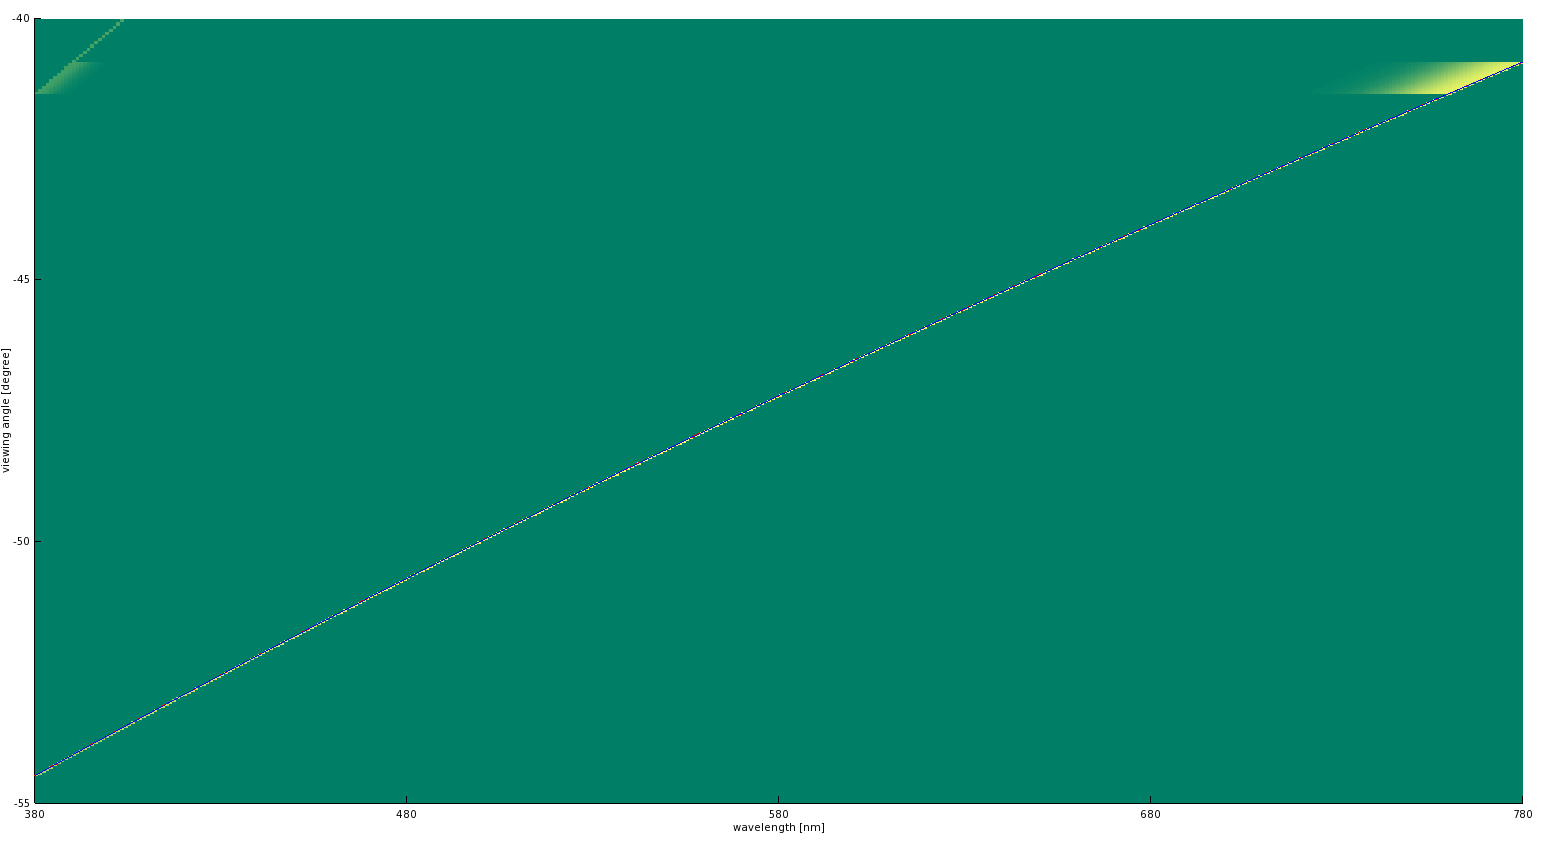
\includegraphics[scale=0.135]{evaluation/bn.png}
    \label{fig:blazneval}
  }
~
  \subfigure[Elaphe grating]{
    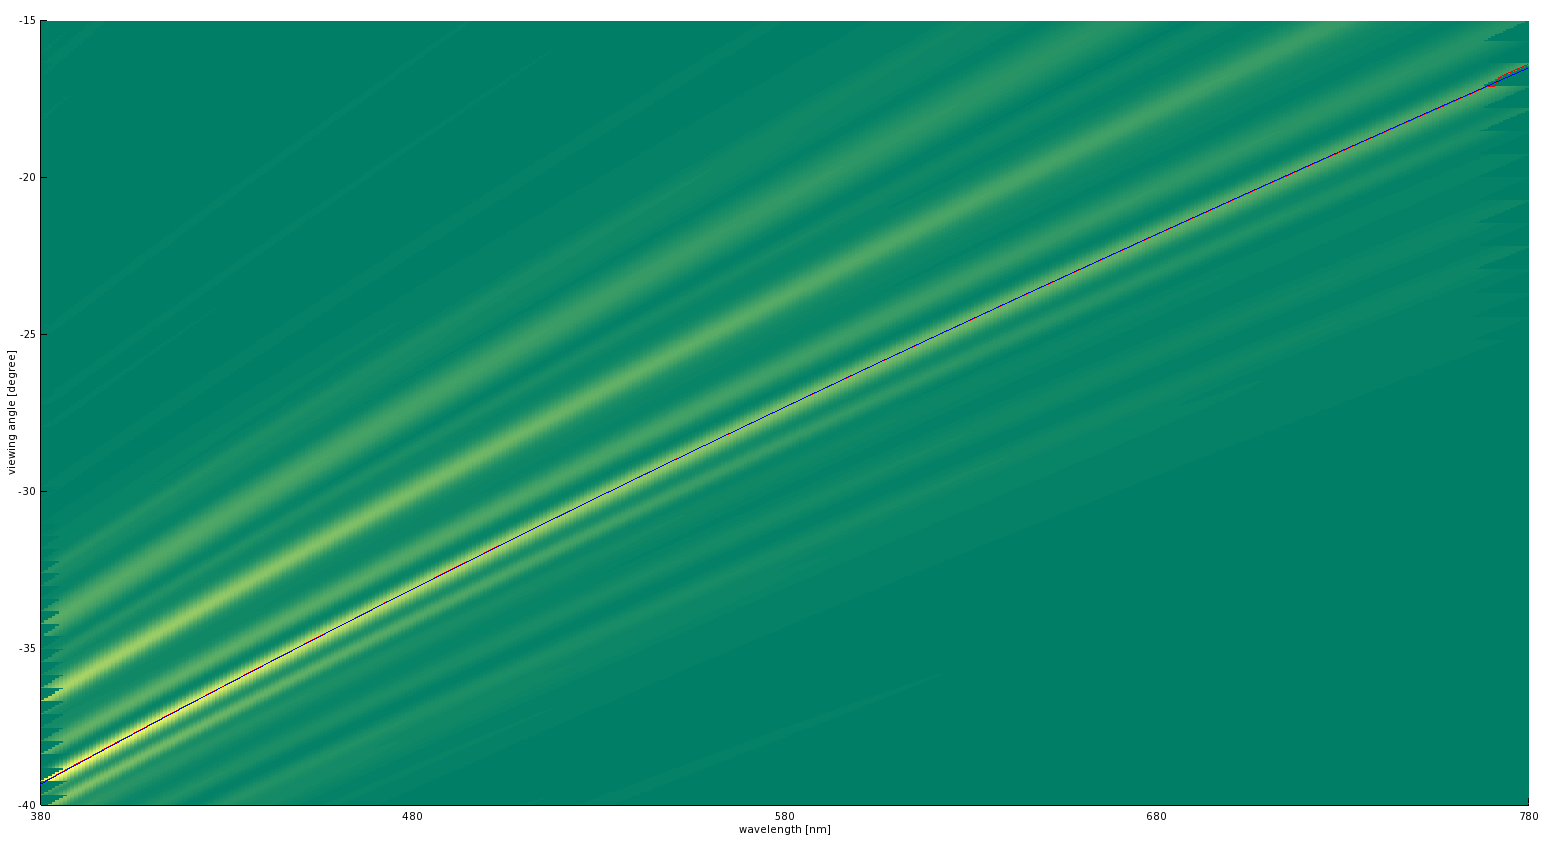
\includegraphics[scale=0.135]{evaluation/en.png}
    \label{fig:elapheneval}
  }
\caption{Reflectance obtained using $N_{min} N_{max}$ optimization apporach}
\label{fig:evaluationdiffshadernminmax}
\end{figure}

Last let us consider the evaluation graphs of the PQ approach $\ref{alg:sincinterpolation}$ in figure $\ref{fig:evaluationdiffshaderpq}$. The PQ approach assumes the given grating being periodically distributed on a shape's surface. For this approach we have plotted evaluation graphs of the Blaze- $\ref{fig:blazepqeval}$ and Elaphe grating $\ref{fig:elaphepqeval}$. For both graphs their response curves have some similarities but also some differences compared to their corresponding grating equation curve. We could say that the response curve of the blaze grating is weakly oscillating around the grating equation curve (blue) but basically following it even there are some outliers. The response curve of the Elpahe grating is not following its corresponding first order grating equation curve rather another response curve for the pq approach. This could be due to the assumption of the PQ approach that a given patch must be periodically distributed along the surface which is actually not that case. Nevertheless, the red curve fits one of the response curves. 

\begin{figure}[H]
  \centering
  \subfigure[Blaze grating]{
    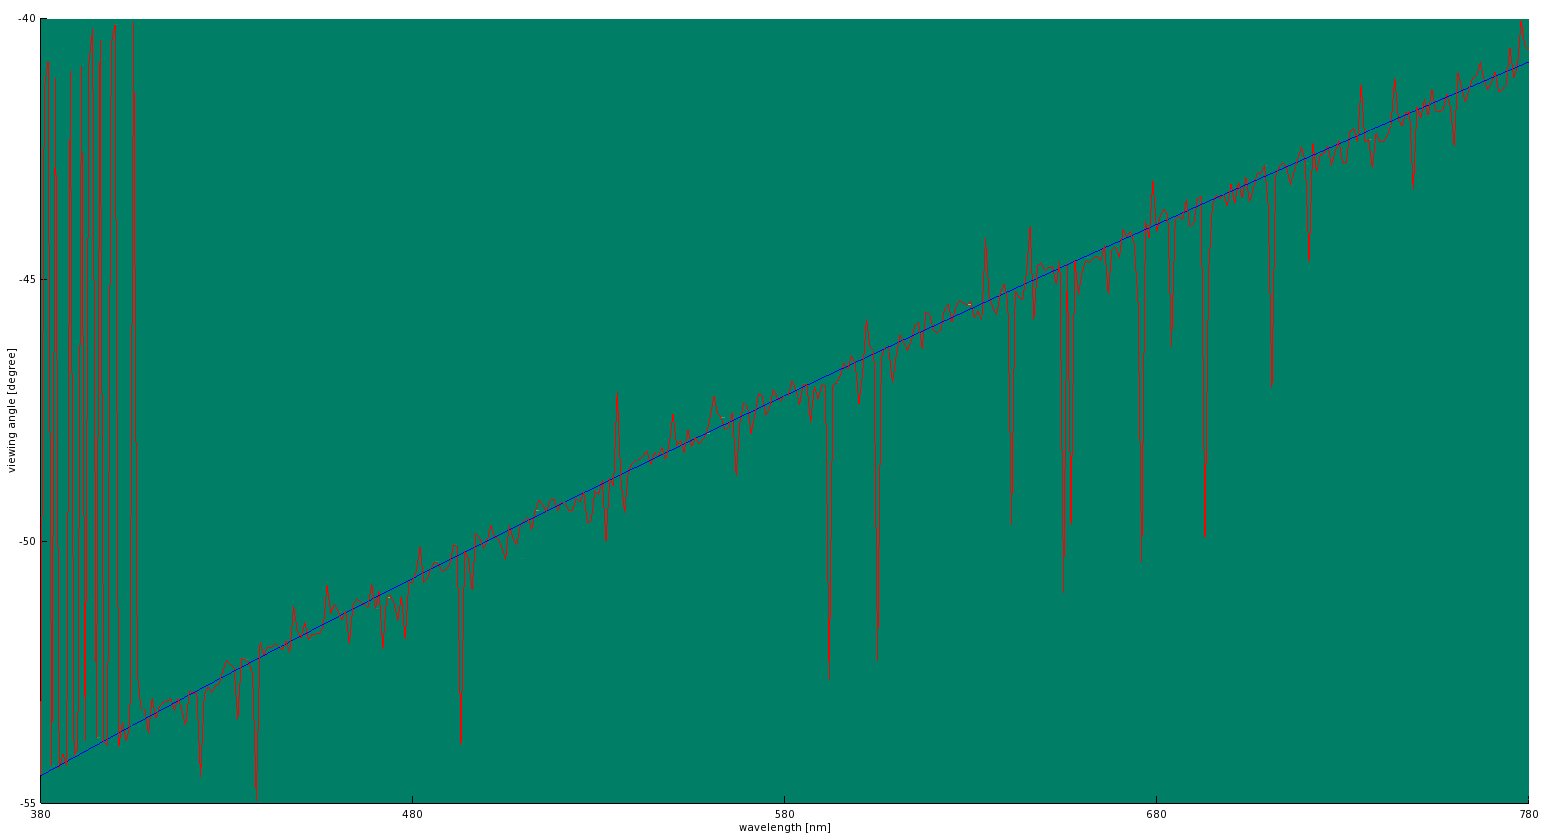
\includegraphics[scale=0.135]{evaluation/bpq.png}
    \label{fig:blazepqeval}
  }
~
  \subfigure[Elaphe grating]{
    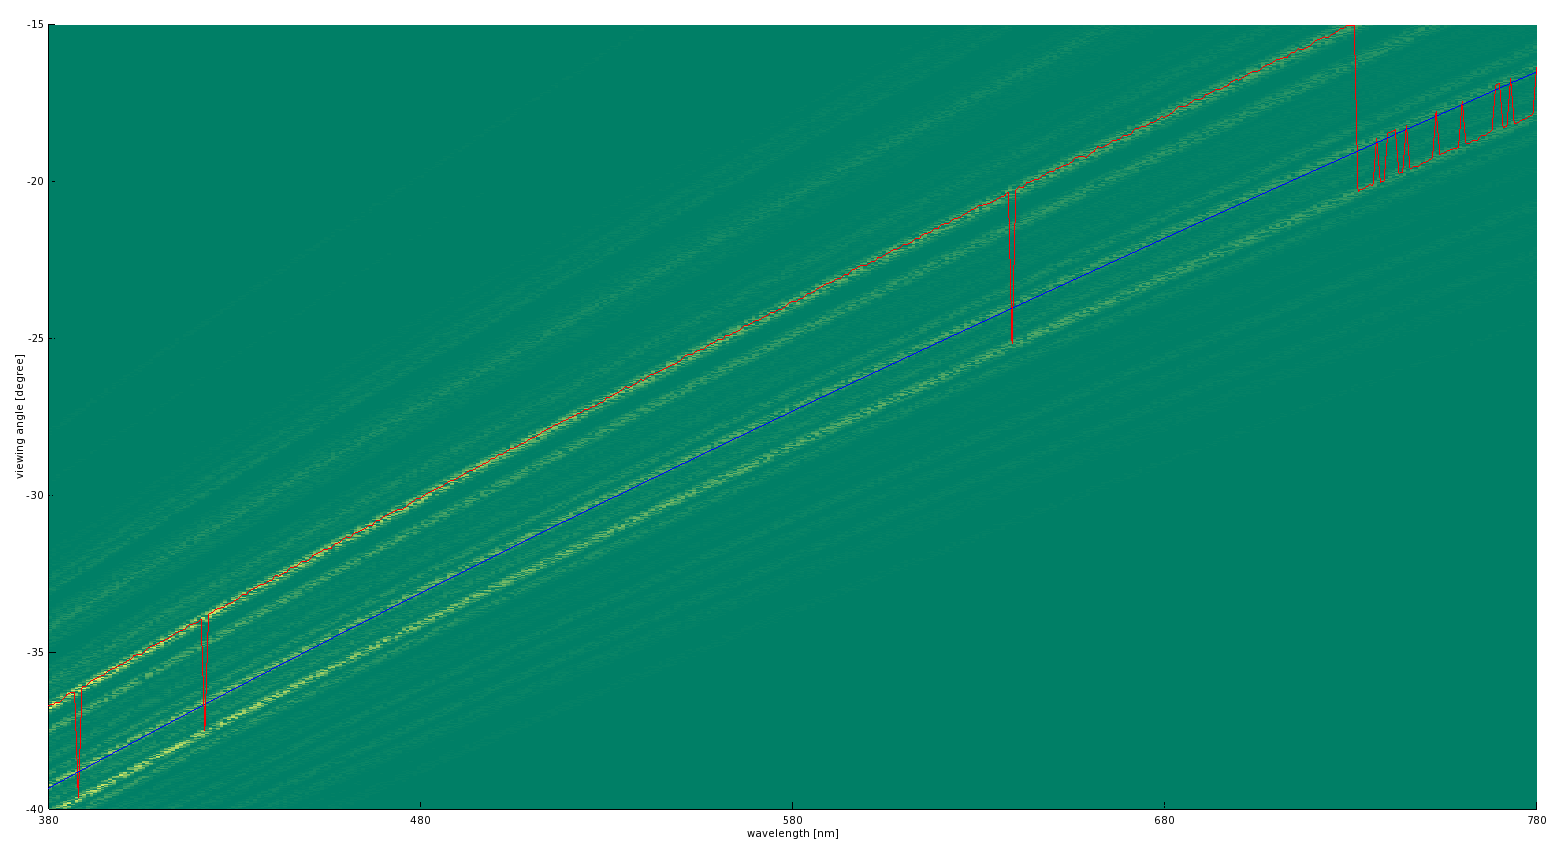
\includegraphics[scale=0.135]{evaluation/epq.png}
    \label{fig:elaphepqeval}
  }
\caption{Reflectance obtained using PQ optimization apporach}
\label{fig:evaluationdiffshaderpq}
\end{figure}

